%-------------------------
%big-picture
%(c) H.Buchmann FHNW 2008
%$Id$
%export TEXINPUTS=${HOME}/fhnw/edu/:${HOME}/fhnw/edu/tinL/config/latex:${HOME}/fhnw/edu/config//:
%-------------------------
\documentclass{beamer}
\usepackage{latex/beamer}
%---------------------
%local defines
%(c) H.Buchmann FHNW 2009
%$Id$
%---------------------
\newcommand{\target} {\beaglebone\xspace}
\newcommand{\targetS}{{\bf BBG}\xspace}
\newcommand{\host}   {{\em Host}\xspace}
\newcommand{\targetroot} {{\bf target-root}\xspace}
\newcommand{\kernel} {{\bf kernel}\xspace}
\renewcommand{\c}{{\bf C}\xspace}
\newcommand{\cpp}{{\bf C++}\xspace}
\newcommand{\posix}{{\bf POSIX}\xspace}

\input{/home/buchmann/latex/dirtree/dirtree.tex}

\title[\unix use]{\unix use}
\begin{document}

\frame{\titlepage}

\begin{frame}{Ziel}{Entwicklung von Programmen auf dem \target}
 \begin{itemize}
  \item alles ist ein File 
  \item Filesysteme
  \begin{itemize}
   \item \cod{mount}
   \item \cod{sshfs}
  \end{itemize}
  \item Cross development
  \begin{itemize}
   \item \host $\leftrightarrow$ \target
   \remark{Keine Toilchain auf dem \target}
  \end{itemize}
 \end{itemize}
\end{frame}

\begin{frame}{Wichtig}
 \begin{itemize}
  \item wo ist was
  \item {\Large Verzeichnisstruktur}
 \end{itemize}
\end{frame}

\section{Alles ist ein File}
\begin{frame}{Alles ist ein File}

\includegraphics{file-bits.jpg}
\begin{itemize}
 \item \cod{\em name} Referenz auf die Bits (Bytes)
 \begin{itemize}
  \item Bits(bytes) der Reihe nach
 \end{itemize}
 \item Files
 \begin{itemize}
  \item Datenquelle
  \begin{itemize}
   \item liefern Daten: Bits(Bytes)
  \end{itemize}
  \item Datensenke
  \begin{itemize}
   \item absorieren Daten: Bits(Bytes)
  \end{itemize}
 \end{itemize}
\end{itemize}
\end{frame}

\begin{frame}{Ein paar Befehle}
 \begin{itemize}
  \item \cod{cat {\em name}}
  \item \cod{hexdump -C {\em name}}
 \end{itemize}
\end{frame}

\begin{frame}{Devices sind auch Files}{z.B. SD-Karte}
 \begin{description}
  \item[\cod{/dev/mmcblk{\bf i}}] $i=0,1,2 ...$
  \remark{Name vom Betriebssystem bestimmt}
  \begin{description}[Datenquelle]
  \item[Datenquelle] \cod{hexdump -C /dev/mmcblk0}
  \item[Datensenke] \cod{cp {\em name} /dev/mmcblk0}
  \remark{Aufpassen}
  \end{description}
 \end{description}
\end{frame}

\begin{frame}{Devices sind auch Files}{z.B Zufallszahlen}
 \begin{description}[\cod{/dev/urandom}]
  \item[\cod{/dev/random}] sammelt das Rauschen: langsam
  \remark{Name vom Betriebssystem bestimmt}
  \begin{description}
   \item[Datenquelle] \cod{hexdump -C /dev/random}
  \end{description}
  \item[\cod{/dev/urandom}] berechnete (Pseudo) Zahlen: schnell
  \begin{description}
   \item[Datenquelle]
   \cod{play -b 16 -e  signed-integer  \textbackslash\\
   -t raw -r 44000 /dev/urandom}
   \remark{der Befehl \cod{play} hat viele Optionen}
  \end{description}
 \end{description}
\end{frame}

\section{Filesystem}
\begin{frame}{Filesystem}{Files f�r Files}
 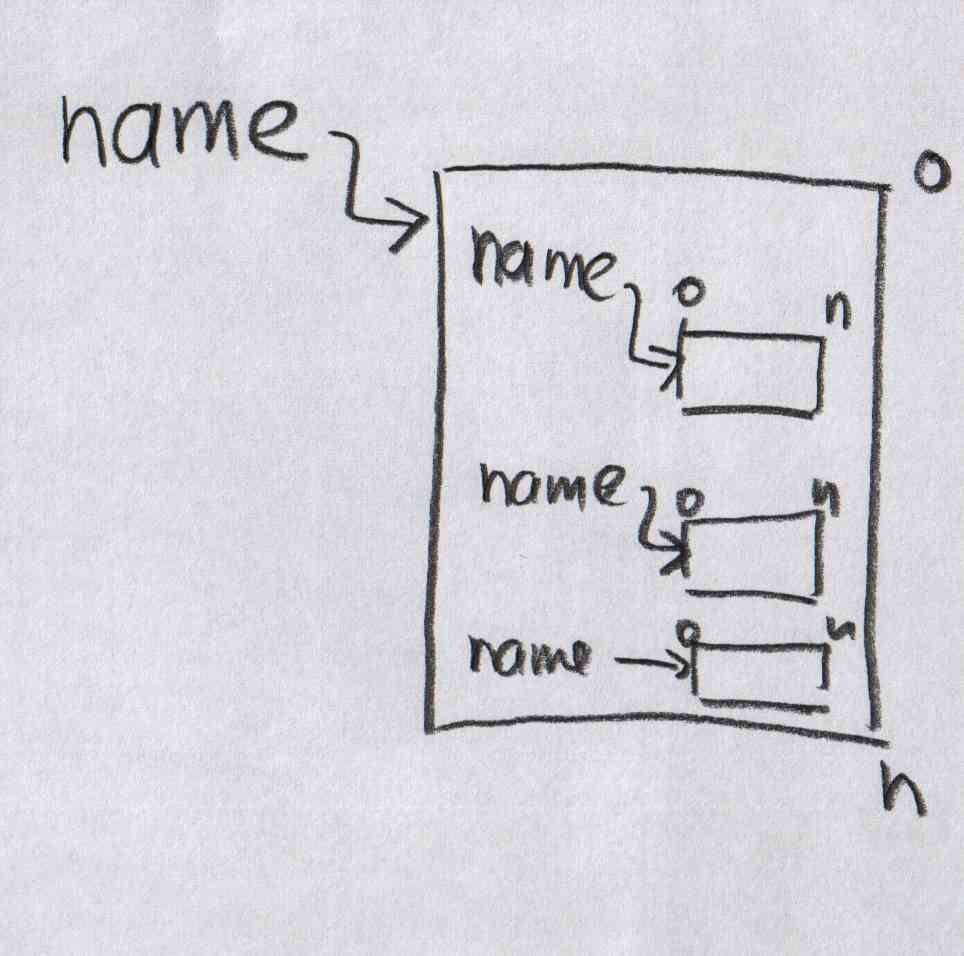
\includegraphics[width=4.5cm]{filesystem.jpg}
 \begin{textblock}{150}(55,30)
  \begin{itemize}
   \item File der weitere Files enth�lt
   \item Verschiedene Filesysteme
   \begin{description}
    \item[vfat] Microsoft 
    \item[ext4] \unix
    \item[...] noch viele andere \\\cod{cat /proc/filesystems}
   \end{description}
  \end{itemize}
 \end{textblock}
\end{frame}

\begin{frame}{Vereichnisstruktur}{Hierarchie}
 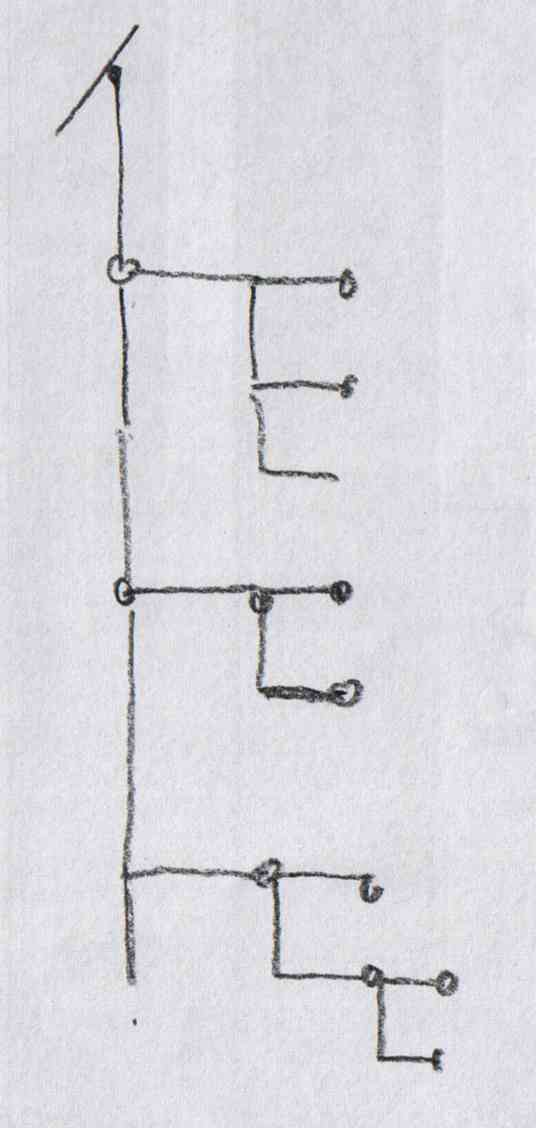
\includegraphics[height=5cm]{dir-tree.jpg}
 \includegraphics[height=5cm]{glbs/2-as-user/doc/tree.png}
 \begin{textblock}{150}(80,65)
  \begin{itemize}
   \item \cod{/} root
   \item ein paar Befehle 
   \begin{itemize}
   \item \cod{ls}, \cod{tree}, \cod{cd}
   \end{itemize}
  \end{itemize}
 \end{textblock}
 \hint[30]{50,40}{Verzeichnisse einer Workstation}
\end{frame}


\begin{frame}{\cod{mount {\em fileSystem} {\em mountPoint}}}
             {Verbindet Filesysteme}
  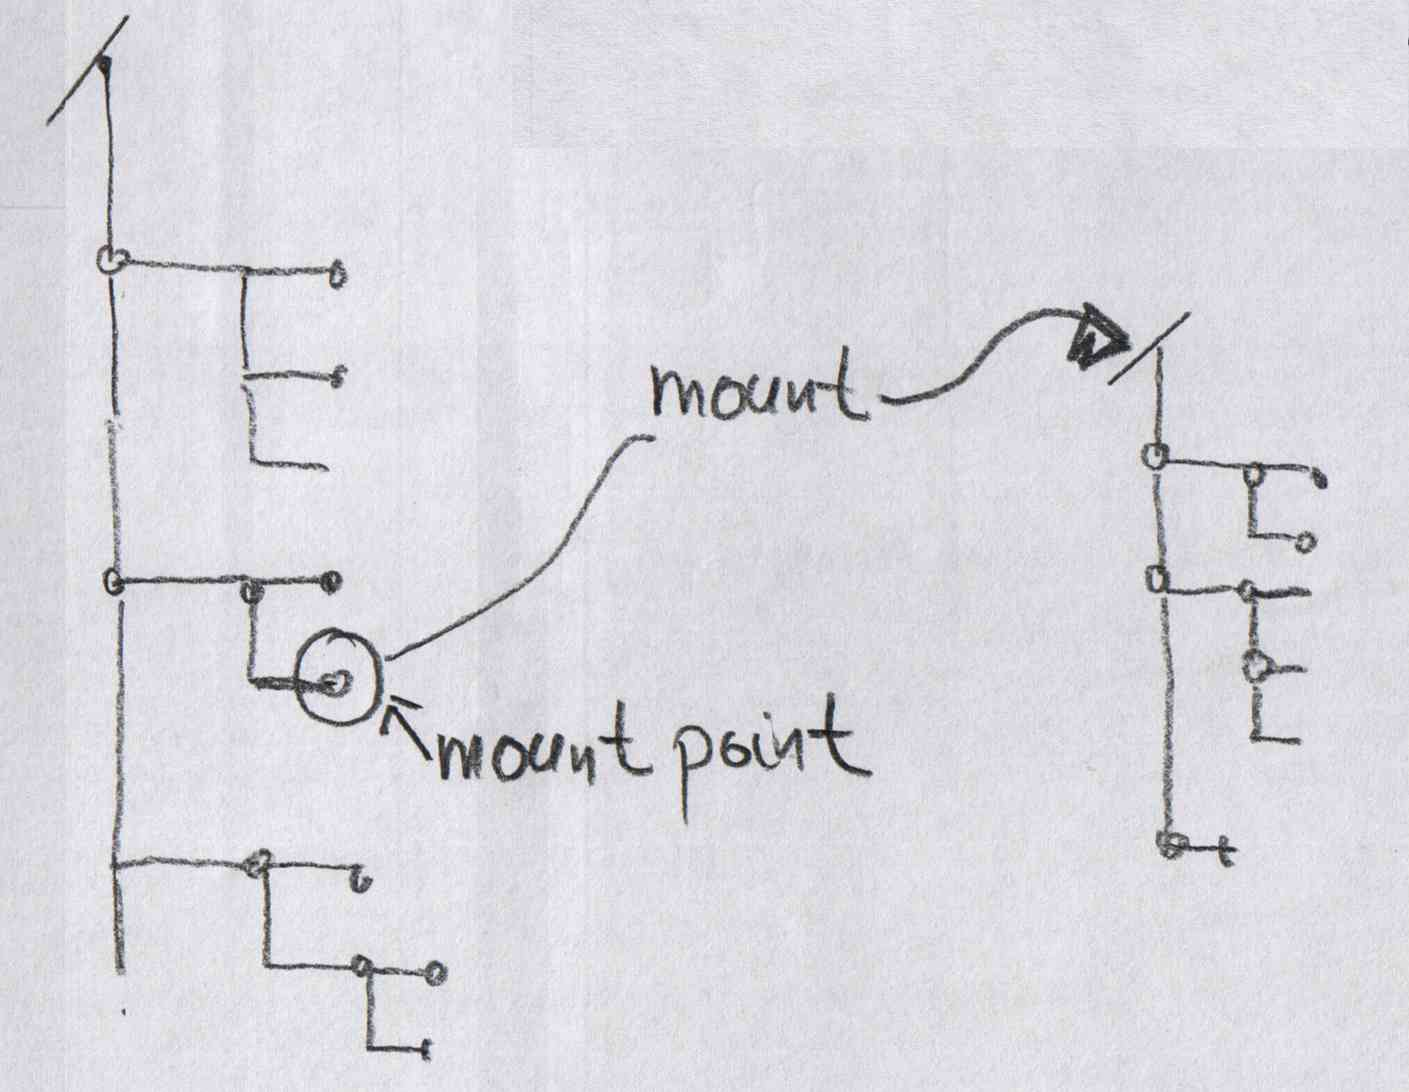
\includegraphics[height=4.5cm]{mount.jpg}
  \begin{textblock}{150}(68,40)
   \begin{itemize}
    \item \cod{mount {\em /dev/mmcblk0p1} \textbackslash \\
    \ \ \ \ {\em mountPoint}}
   \end{itemize}
  \end{textblock}
  \remark{Sieht wie ein normales Verzeichnis aus}
\end{frame}

\begin{frame}{\cod{sshfs user@host mountPoint}}{via \cod{ssh}}
 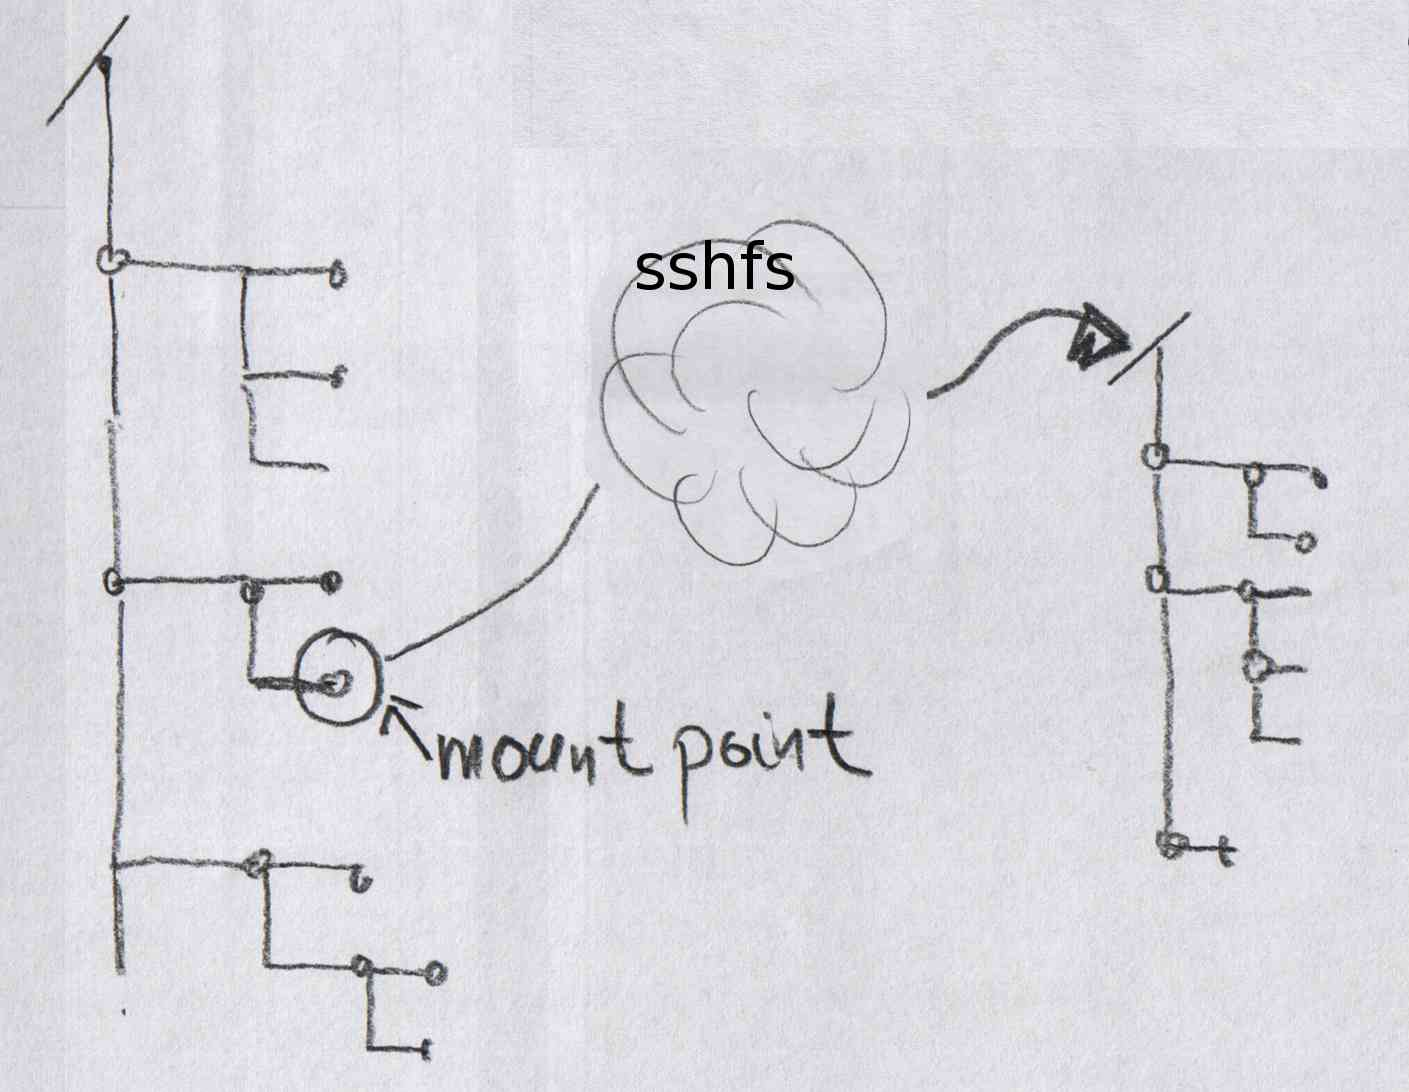
\includegraphics[height=4.5cm]{sshfs.jpg}
   \begin{textblock}{150}(68,40)
   \begin{itemize}
    \item braucht \cod{ssh}
   \end{itemize}
  \end{textblock}
  \remark{Sieht wie ein normales Verzeichnis aus}
\end{frame}

\section{Cross development}
\begin{frame}{Verzeichnisstruktur}{\host \target}
 \begin{block}{Host} 
 \dirtree{%
  .1 devel \DTcomment{somewhere on the host}.
  .2 config.
  .3 Makefile \DTcomment{for making \target executables}.
  .2 java \DTcomment{source}.
  .2 src  \DTcomment{c c++}.
  .2 tc    \DTcomment{normally a link}.
  .2 {\bf work} \DTcomment{connected with \target {\em current dir}}.
 }
 \end{block}
 \begin{block}{\target} 
 \dirtree{%
  .1 user \DTcomment{somewhere on the \target}.
  .2 {\bf work} \DTcomment{connected with \host {\em current dir}}.
 }
 \end{block}
\end{frame}


\section{}
\begin{frame}{Aufgaben}
 \begin{itemize}
  \item Verbindung mit \target via \cod{ssh}
  \item upgrade \cod{pacman -Suy}
  \item {\em user} auf \target \cod{useradd}
  \item {\em toolchain} auf \host
  \item mount \host auf \target mit \cod{sshfs}
  \item \cod{HelloWorld.java}, \cod{hello-world-cpp.cc}, \cod{hello-world-c.c}, 
        \cod{primes.cc}\\
  auf \target
 \end{itemize}
\end{frame}
\end{document}

